\todo[inline]{PROBLEM - SYSTEM}

\begin{figure}
\centering 
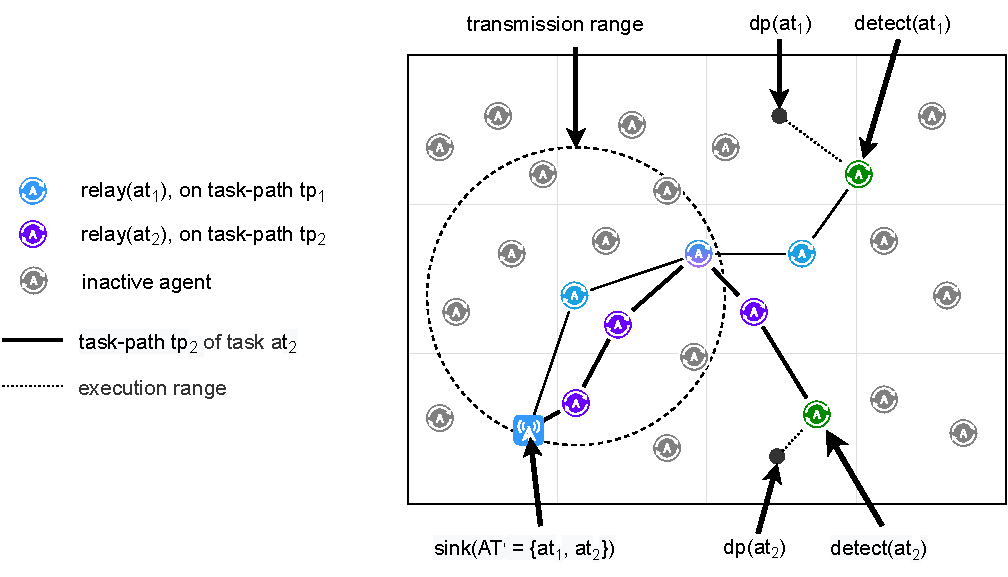
\includegraphics[width=0.9\linewidth]{grid_concept}
\caption[WSN deployment terminology]{WSN deployment terminology}
\label{fig:gridconcept}
\end{figure}

\subsection{System definition}
\todo[inline]{This is a summary of our previous work, so keep it short and reference stuff}
Given a geographical area to monitor, we can overlay a two dimensional grid of real numbers, allowing us to associate a deployed set of nodes, or agents, $\setAgents{}{}$, with a corresponding location, $\formalVarLocation{}{} \in \formalSetLocation{}{}$. on the grid. This describes the \textit{deployment configuration} of those agents, a mapping from agents to real valued tuples representing their location,  $\formalDeployment{}{}$.

An \textit{atomic task} $\varAtomicTask{}{}$ is a task to take a measurement at a target location, the \textit{demand point} for that measurement $\functionTaskDemandPoint{}{}$, which must be in range of its relevant sensor. A \textit{composite task}, is composed of $N$ atomic tasks $\varCompositeTask{}{} = \lbrace \varAtomicTask{i}{} \rbrace_{i=0}^N$ where for each of the $i\in N$ grid blocks of the systems geographical grid area. At at time $\varTime{}{}$, each agent carrying out a measurement task has a certain amount of resources $\varResource{}{}$, in this case energy, assigned to completion of tasks of that type, given by $\formalTaskResourceAllocation{}{}$
\todo[inline]{Summarise system definition}
We can therefore define the system as a tuple $s = (PG, CG, \setAtomicTask{}{}, \setCompositeTask{}{}, \setResource{}{}, ar, tg)$, where
\begin{itemize}
 \item $PG$ is a set of parent agents,
 \item $CG$ is a set of child agents,
 \item $TP$ is a set of atomic task types,
 \item $\setCompositeTask{}{} \subseteq \powerSetSymbol{\setAtomicTask{}{}}{}{}$ is the set of composite task types (sets of atomic task types) that occur in the system,
 \item $\setResource{}{}$ is a set of resources needed to perform tasks,
 \item $ar: CG \times R \rightarrow R>=0$ is a mapping from each child agent and each resource to the amount of that resource that
the agent possesses.
\item $tg: \setCompositeTask{}{} \rightarrow 2^{PG}$ is a mapping from each composite task type to the group of parent agents that receive and ensure the completion of tasks of that type.
\end{itemize}

\subsection{Node roles and task arcs}
%%%%%%%%%%%%%%%%%%%%%%%%%%%%%%%%%%%%%%%%%%%%
\newcommand{\formalSinkRole}[2]{
	\functionFormal{sink}
	{\setCompositeTask{}{} \times \setAgents{}{}}
	{\setAgents{}{}}
}
\newcommand{\formalSenseRole}[2]{
	\functionFormal{sense}
	{\setAtomicTask{}{} \times \setAgents{}{}}
	{\powerSetAgents{}{}}
}
\newcommand{\formalActiveRole}[2]{
	\functionFormal{active}
	{\setAtomicTask{}{} \times \setAgents{}{}}
	{\powerSetAgents{}{}}
}
\newcommand{\formalIdleRole}[2]{
	\functionFormal{idle_{\setTime{}{}}}
	{\setAgents{}{}}
	{\setAgents{}{}}
}
\newcommand{\formalSleepRole}[2]{
	\functionFormal{sink_{\setTime{}{}}}
	{\setAgents{}{}}
	{\setAgents{}{}}
}
\newcommand{\functionSinkRole}[2]{\functionSignature{sink}{\varCompositeTask{}{}, \setAgents{}{}}}
	
\newcommand{\functionSenseRole}[2]{\functionSignature{sense}{\varAtomicTask{}{}, \setAgents{}{}}}
\newcommand{\functionActiveRole}[2]{\functionSignature{active}{\varAtomicTask{}{}, \setAgents{}{}}}
\newcommand{\functionIdleRole}[2]{\functionSignature{idle}{\varAtomicTask{}{}, \setAgents{}{}}}
\newcommand{\functionSleepRole}[2]{\functionSignature{sleep}{\varAtomicTask{}{}, \setAgents{}{}}}

We can distinguish agents by the role they play in a given atomic task.
\begin{itemize}
	\item A \textit{sink node} of a composite task $\varAtomicTask{}{}$ is the agent that first receives the composite task , and will broadcast the results, $\formalSinkRole{}{}$.
	\item A \textit{sensing node} is the agent that executes the atomic task and so performs the sensor measurement, $\formalSenseRole{}{}$.
	\item An \textit{active node} is an agent that participates in sub-allocating, or routing, that task, but is neither a sink agent nor a sensing agent, $\formalActiveRole{}{}$..
	\item An \textit{idle node} does not participate in the specific task, but is for other tasks during a time period $\setTime{}{}$, $\formalIdleRole{}{}$.
	\item An \textit{sleeping node} does not participate in any of the tasks in the system during a time period $\setTime{}{}$, $\formalSleepRole{}{}$.
\end{itemize}
With these roles in mind, we can now define the  \textit{atomic task arc} as a mapping of atomic tasks to ordered sequence of agents $\formalTaskArc{}{}$ that each atomic task $\varAtomicTask{}{}$ is sub-allocated to. The first agent is the agent that has received the initial composite task, and the last agent is the agent that executes the atomic task such that, 
$\functionTaskArc{}{} = \lbrace \varSinkAgent{}{}, \varActiveAgent{i}{}, \varSensingAgent{}{} \rbrace_{i=1}^{n}$. Note, generally communications in WSN networks are multi-hop due to the limited broadcast range of nodes, therefore are $n>0$ active agents sub-allocating the task between the sink and sensing agents.

